\documentclass{article}
\usepackage{tikz}
\usetikzlibrary{calc,matrix,decorations.markings,decorations.pathreplacing}
\usetikzlibrary{arrows,shapes,chains}
\begin{document}

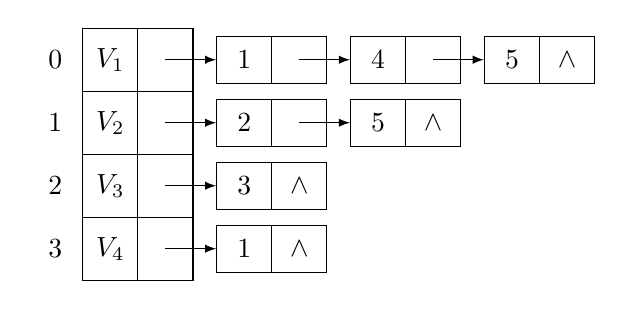
\begin{tikzpicture}[nodes in empty cells,
      nodes={minimum width=0.7cm, minimum height=0.6cm}]
    \node(0){0};
    \node[draw,rectangle,node distance=0.7cm,right of=0,minimum height=0.8cm](n0){$V_1$} ;
    \node[rectangle,draw,right of=n0,node distance=0.7cm,minimum height=0.8cm](n1){};
    \node[rectangle,draw, right of=n1](n2){1};
    \node[rectangle,draw, right of=n2,node distance=0.7cm](n3){};
    \node[rectangle,draw, right of=n3](n4){4};
    \node[rectangle,draw, right of=n4,node distance=0.7cm](n5){};
    \node[rectangle,draw, right of=n5](n6){5};
    \node[rectangle,draw, right of=n6,node distance=0.7cm](n7){$\wedge$};
    \draw[-latex] (n1.center) -- (n2.west);
    \draw[-latex] (n3.center) -- (n4.west);
    \draw[-latex] (n5.center) -- (n6.west);

    \node(1)[node distance=0.8cm, below of=0]{1};
    \node[draw,rectangle,node distance=0.7cm,right of=1,minimum height=0.8cm](n8){$V_2$} ;
    \node[rectangle,draw,right of=n8,node distance=0.7cm,minimum height=0.8cm](n9){};
    \node[rectangle,draw, right of=n9](n10){2};
    \node[rectangle,draw, right of=n10,node distance=0.7cm](n11){};
    \node[rectangle,draw, right of=n11](n12){5};
    \node[rectangle,draw, right of=n12,node distance=0.7cm](n13){$\wedge$};
    \draw[-latex] (n9.center) -- (n10.west);
    \draw[-latex] (n11.center) -- (n12.west);

    \node(2)[node distance=0.8cm, below of=1]{2};
    \node[draw,rectangle,node distance=0.7cm,right of=2,minimum height=0.8cm](n14){$V_3$} ;
    \node[rectangle,draw,right of=n14,node distance=0.7cm,minimum height=0.8cm](n15){};
    \node[rectangle,draw, right of=n15](n16){3};
    \node[rectangle,draw, right of=n16,node distance=0.7cm](n17){$\wedge$};
    \draw[-latex] (n15.center) -- (n16.west);

    \node(3)[node distance=0.8cm, below of=2]{3};
    \node[draw,rectangle,node distance=0.7cm,right of=3,minimum height=0.8cm](n18){$V_4$} ;
    \node[rectangle,draw,right of=n18,node distance=0.7cm,minimum height=0.8cm](n19){};
    \node[rectangle,draw, right of=n19](n20){1};
    \node[rectangle,draw, right of=n20,node distance=0.7cm](n21){$\wedge$};
    \draw[-latex] (n19.center) -- (n20.west);

\end{tikzpicture}

\end{document}
